\section{Jerarquía de Memoria}
Existen distintos niveles de almacenamiento, todos con sus pros y contras.

\begin{figure}[h]
  \centering
  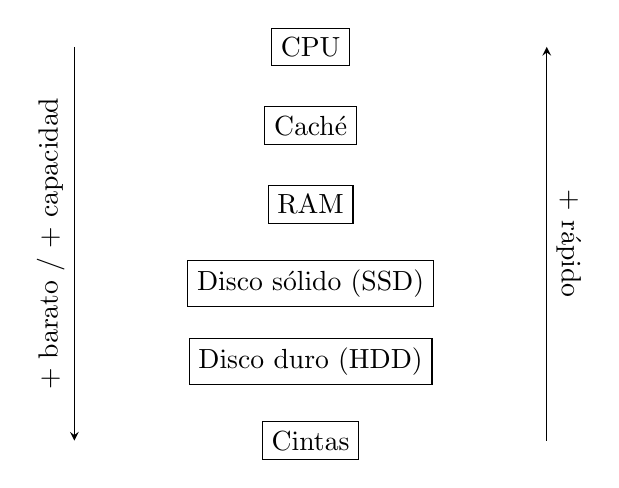
\begin{tikzpicture}
    \node[draw, rectangle] (cpu) {CPU};
    \node[draw, rectangle, below of=cpu] (cache) {Caché};
    \node[draw, rectangle, below of=cache] (ram) {RAM};
    \node[draw, rectangle, below of=ram] (ssd) {Disco sólido (SSD)};
    \node[draw, rectangle, below of=ssd] (hdd) {Disco duro (HDD)};
    \node[draw, rectangle, below of=hdd] (tape) {Cintas};

    \draw[-stealth] (-3,0) -- (-3,-5) node[above, midway, rotate=90] {+ barato / + capacidad};
    \draw[-stealth] (3,-5) -- (3,0) node[above, midway, rotate=270] {+ rápido};
  \end{tikzpicture}
  \caption{Jerarquía de Memoria}
\end{figure}

Cabe destacar que en la jerarquía tenemos memoria volátil y no volátil. La memoria volátil es la memoria que una vez se desconecta su energía o se apaga, pierde todos sus datos, mientras que la no volátil, una vez desconectada su energía es capaz de mantener sus datos.
\begin{itemize}
  \item Volátil:
  \begin{itemize}
    \item CPU
    \item Caché
    \item RAM (Memoria principal)
  \end{itemize}
  \item No volátil:
  \begin{itemize}
    \item Disco sólido (SSD)
    \item Disco duro (HDD)
    \item Cintas
  \end{itemize}
\end{itemize}

Para las bases de datos, claramente la parte más importante de esta jerarquía sería el almacenamiento persistente que se usa hoy en día: Los discos duros magnéticos y los discos sólidos.

\section{El disco duro}
El interior de un disco duro se ve así
\begin{figure}[h]
  \centering
  \includegraphics[width=0.7\textwidth]{img/disk_anatomy.png}
  \caption{Interior de un disco duro}
\end{figure}

\subsection{Sectores, bloques y páginas}
Cuando trabajamos con un disco duro, se usan estos términos para hablar de la ubicación de datos dentro de este.
\begin{itemize}
  \item Sector: Un sector es la unidad física mínima de almacenamiento.
  \item Bloque: Un bloque es la unidad lógica mínima de almacenamiento en disco.
  \item Página: Una página es la unidad lógica mínima de almacenamiento en el sistema.
\end{itemize}

\subsection{Demora en búsqueda de datos (y escritura)}
Si se desea obtener un cierto dato desde un disco duro mecánico, es esperable que tome un poco de tiempo. Esto debido a los distintos pasos que se deben realizar para llegar al dato deseado. El tiempo total esta dado por
\[ \text{Tiempo total} = \text{Tiempo de búsqueda} + \text{Retraso rotacional} + \text{Velocidad de transferencia} \]

\begin{itemize}
  \item Tiempo de búsqueda: Tiempo que se demora el disco en posicionar la cabeza en el track correspondiente (3ms - 15ms promedio).
  \item Retraso rotacional: Tiempo que se demora en rotar el disco al primer sector (2ms - 7ms promedio).
  \item Velocidad de transferencia: Tiempo que toma leer los sectores, incluyendo espacios entremedio (depende del tamaño de los datos).
\end{itemize}

A la hora de escribir en el bloque, la demora es similar (o un poco mayor). Para modificar un bloque se debe primero leer el bloque, luego hacer las modificaciones a dicho bloque en memoria, para finalmente escribir el bloque usando el contenido presente en memoria.


\subsection{Optimizaciones a la hora de usar el disco}
Considerando que hacer cosas en el disco es bastante lento, lo ideal seria optimizar lo más posible el proceso. De esta forma, nuestro sistema tardará menos en responder consultas o escribir información nueva.


\makeobservationbox{Localidad de los datos}{
  Si las tuplas $t$ y $t'$ son parte de la misma relación $R$, entonces se debe almacenar $t$:
  \begin{itemize}
    \item En el mismo bloque que $t'$. Si no\dots
    \item En el mismo track que $t'$. Si no\dots
    \item En el mismo cilindro que $t'$. Si no\dots
    \item En el cilindro contiguo a $t'$.
  \end{itemize}
}

\makeobservationbox{Pre-fetch}{
  La idea es adivinar y traer bloques que se predice que serán solicitados en el futuro. Para esto, si por ejemplo, se solicita el bloque $k$, traer los bloques contiguos a $k$, como $k+1, k+2, k+3, \ldots, k+N$, donde $N$ es definido por el usuario (cuanto mayor $N$, mayor será el costo de la optimización. Usar con cautela).
}

\makeobservationbox{Planificación del disco}{
  Dada una secuencia de solicitudes $o_1, \ldots, o_n$ al disco, reordenar las solicitudes a $o_{i_1}, \ldots, o_{i_n}$ de tal forma que se minimice el tiempo total.
  
  Esto por ejemplo, se puede hacer reordenando las solicitudes de forma tal que se escriban todas las cosas en lugares cercanos del disco, para moverse una sola vez a otro sitio, en lugar de ir y volver varias veces (mover el cabezal consume mucho tiempo)
}

\makeobservationbox{Múltiples discos}{
  Distribuir tuplas en múltiples discos, para así tener acceso concurrente a las relaciones y tuplas.
  
  En otras palabras, la idea es que podamos usar varios discos a la vez para leer la información más rápido. Esto es posible solamente si los datos se encuentran distribuidos en múltiples discos. En un solo disco debemos esperar a que el cabezal lea un dato y después avance al siguiente. Si tenemos, por ejemplo, 8 discos, es posible leer 8 tuplas en el tiempo que nos toma leer una desde un solo disco. 
}

\makeobservationbox{Múltiples copias (mirroring)}{
  Principio muy similar al anterior. Consiste en mantener múltiples copias de los datos en varios discos. Esto genera redundancia, por lo que ante fallas se logra mantener disponibilidad de los datos (o incluso hacer que una falla no sea catastrófica). Esto también aumenta la velocidad de lectura de los datos, aunque genera mayor lentitud a la hora de escribir (ya que todos los discos que tengan copias tendrán que sincronizar los datos. Escribir un dato implicará escribir en varios lugares.).
}

\section{Organizando los datos con páginas}
Ahora que comprendemos como usar el disco correctamente, toca responder la pregunta siguiente: \textit{¿Cómo almacenamos las distintas tuplas de una relación en el disco?}. ¡Aquí es donde las páginas juegan un rol fundamental!

Una página (sistema) corresponde a un bloque en el disco. Cada relación corresponde a un set de páginas que contienen un subconjunto de tuplas. Esto entrega un manejo granular del contenido del disco, optimiza el acceso al disco y facilita el manejo de las transacciones.

\subsection{Heapfiles}
Un heapfile es una estructura de datos diseñada para almacenar relaciones en páginas.

Para almacenar una tupla en un heapfile, podemos escribir primero un directorio, el cual nos indica a que offset del disco dirigirnos para obtener un cierto atributo de la tupla. Eso se ve más o menos así.

\begin{figure}[h]
  \centering
  \begin{tikzpicture}
    \draw[draw=black] (0,0) rectangle (0.2,1) node[pos=.5] (dir1) {};
    \draw[draw=black] (0.2,0) rectangle (0.4,1) node[pos=.5] (dir2) {};
    \draw[draw=black] (0.4,0) rectangle (0.6,1) node[pos=.5] (dir3) {};
    \draw[draw=black] (0.6,0) rectangle (0.8,1) node[pos=.5] (dir4) {};
    \draw[draw=black] (0.8,0) rectangle (1,1) node[pos=.5] (dir5) {};
    \draw[draw=black] (1,0) rectangle (3,1) node[pos=.5] (att1) {\texttt{att$_1$}};
    \draw[draw=black] (3,0) rectangle (5,1) node[pos=.5] (att2) {\texttt{att$_2$}};
    \draw[draw=black] (5,0) rectangle (7,1) node[pos=.5] (att3) {\texttt{att$_3$}};
    \draw[draw=black] (7,0) rectangle (9,1) node[pos=.5] (att4) {\texttt{att$_4$}};
    \draw[draw=black] (9,0) rectangle (11,1) node[pos=.5] (att5) {\texttt{att$_5$}};
    
    \draw [decorate,decoration={brace,amplitude=5pt,raise=4ex}] (1,.5) -- (0,.5) node[midway,yshift=-3em]{Directorio};
    \draw[-Stealth] (dir1.north)+(0,.1) -- ++(0,.5) -| (att1.north);
    \draw[-Stealth] (dir2.north)+(0,.1) -- ++(0,.6) -| (att2.north);
    \draw[-Stealth] (dir3.north)+(0,.1) -- ++(0,.7) -| (att3.north);
    \draw[-Stealth] (dir4.north)+(0,.1) -- ++(0,.8) -| (att4.north);
    \draw[-Stealth] (dir5.north)+(0,.1) -- ++(0,.9) -| (att5.north);

  \end{tikzpicture}
  \caption{Ejemplo de una tupla en un heapfile.}
\end{figure}

Luego, como deseamos almacenar varias tuplas, lo ideal sería darles un identificador. A esto se le llama \textit{``Record ID''}. En general, una buena elección de RID es $(\text{PageID}, \text{NumSlot})$. Ahora, para almacenar varias tuplas, hay dos approachs: Almacenar tuplas de largo fijo y almacenar tuplas de largo variable.

\begin{figure}[h]
  \centering
  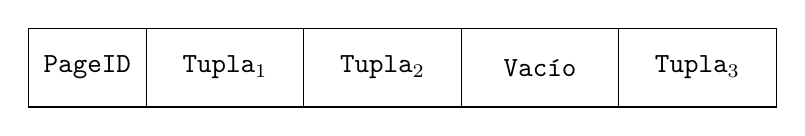
\begin{tikzpicture}
    \draw[draw=black] (0,0) rectangle (1.5,1) node[pos=.5] (pageid) {\texttt{PageID}};
    \draw[draw=black] (1.5,0) rectangle (3.5,1) node[pos=.5] (slot1) {\texttt{Tupla$_1$}};
    \draw[draw=black] (3.5,0) rectangle (5.5,1) node[pos=.5] (slot2) {\texttt{Tupla$_2$}};
    \draw[draw=black] (5.5,0) rectangle (7.5,1) node[pos=.5] (slot3) {\texttt{Vacío}};
    \draw[draw=black] (7.5,0) rectangle (9.5,1) node[pos=.5] (slot4) {\texttt{Tupla$_3$}};
    
    % \draw [decorate,decoration={brace,amplitude=5pt,raise=4ex}] (1,.5) -- (0,.5) node[midway,yshift=-3em]{Directorio};
    % \draw[-Stealth] (dir1.north)+(0,.1) -- ++(0,.5) -| (att1.north);
    % \draw[-Stealth] (dir2.north)+(0,.1) -- ++(0,.6) -| (att2.north);
    % \draw[-Stealth] (dir3.north)+(0,.1) -- ++(0,.7) -| (att3.north);
    % \draw[-Stealth] (dir4.north)+(0,.1) -- ++(0,.8) -| (att4.north);
  \end{tikzpicture}
  \caption{Ejemplo de una página con tuplas de largo fijo.}
\end{figure}

\begin{figure}[h]
  \centering
  \begin{tikzpicture}
    \draw[draw=black] (0,0) rectangle (1.5,1) node[pos=.5] (pageid) {\texttt{Header}};
    \draw[draw=black] (1.5,0) rectangle (1.7,1) node[pos=.5] (dir1) {};
    \draw[draw=black] (1.7,0) rectangle (1.9,1) node[pos=.5] (dir2) {};
    \draw[draw=black] (1.9,0) rectangle (2.1,1) node[pos=.5] (dir3) {};
    \draw[draw=black] (2.1,0) rectangle (5,1) node[pos=.5] (slot1) {\texttt{Vacío}};
    \draw[draw=black] (5,0) rectangle (7,1) node[pos=.5] (slot2) {\texttt{Slot$_3$}};
    \draw[draw=black] (7,0) rectangle (8,1) node[pos=.5] (slot3) {\texttt{Slot$_2$}};
    \draw[draw=black] (8,0) rectangle (9.5,1) node[pos=.5] (slot4) {\texttt{Slot$_1$}};
    
    \draw [decorate,decoration={brace,amplitude=5pt,raise=4ex}] (2.1,.5) -- (1.5,.5) node[midway,yshift=-3em]{Directorio};
    \draw[-Stealth] (dir1.north)+(0,.1) -- ++(0,.9) -| (8,1);
    \draw[-Stealth] (dir2.north)+(0,.1) -- ++(0,.8) -| (7,1);
    \draw[-Stealth] (dir3.north)+(0,.1) -- ++(0,.7) -| (5,1);
  \end{tikzpicture}
  \caption{Ejemplo de una página con tuplas de largo variable.}
\end{figure}
\pagebreak

La última pregunta que queda por responder es como almacenar una misma relación en varias páginas. Para mantener el orden, una forma de hacerlo es por medio de overflow pages. Esto puede conducir a una base de datos lenta e ineficiente, por lo que se recomienda usar con discreción.

\begin{figure}[h]
  \centering
  \begin{tikzpicture}
    \draw[draw=black] (0,0) rectangle (1,1) node[pos=.5] (page1) {\texttt{Page}};
    \draw[draw=black] (1,0) rectangle (2,1) node[pos=.5] (page2) {\texttt{Page}};
    \draw[draw=black] (2,0) rectangle (3,1) node[pos=.5] (page3) {\texttt{Page}};
    \draw[draw=black] (3,0) rectangle (4,1) node[pos=.5] (page4) {\texttt{Page}};
    \draw[draw=black] (4,0) rectangle (5,1) node[pos=.5] (page5) {\texttt{Page}};
    \draw[draw=black] (5,0) rectangle (6,1) node[pos=.5] (page6) {\texttt{Page}};
    \draw[draw=black] (3,-1) rectangle (4,-2) node[pos=.5] (pageoverflow) {\texttt{Page}};
    
    \draw[-Stealth]  (page4) -- (pageoverflow);
  \end{tikzpicture}
  \caption{Ejemplo de overflow page.}
\end{figure}


\section{Buffer Manager}
El buffer manager es el mediador entre el disco y la memoria principal. Cuenta con una cantidad restringida de la memoria RAM del sistema en donde se ejecuta la base de datos. Este componente se encarga de llevar las páginas del disco a la memoria bajo demanda, y es también responsable de decir que páginas deben ser eliminadas de la memoria cuando se encuentra lleno.

\begin{figure}[h]
  \centering
  \includegraphics[width=\textwidth, trim=100 350 100 280, clip]{graphs/buffer_manager.pdf}
  \caption{Buffer Manager}
\end{figure}

Aqui, cada frame tiene dos variables:
\begin{itemize}
  \item \texttt{\#pin}: Cantidad de procesos que están usando actualmente la página.
  \item \texttt{dirty}: Si el contenido de la memoria ha cambiado con respecto al contenido en el disco.
\end{itemize}

Luego, se deben exponer dos funciones para que los procesos de la base de datos puedan usar el buffer manager.
\begin{itemize}
  \item \texttt{pin(pageno)}
  \begin{enumerate}
    \item Solicitar la página \texttt{pageno} al buffer manager.
    \begin{itemize}
      \item Si la página no se encuentra en memoria, se debe seleccionar un frame vacío, traer la página a la memoria y cargar en el frame vacio. Finalmente, al frame se le asigna \texttt{\#pin = 1} y \texttt{dirty = false}.
      \item Si la página ya está en memoria, simplemente \texttt{\#pin += 1}.
    \end{itemize}
    \item Retornar referencia al frame que contiene a \texttt{pageno}
  \end{enumerate}
  \item \texttt{unpin(pageno, dirty)}
  \begin{enumerate}
    \item Solicitar la liberación de la página \texttt{pageno} al buffer manager.
    \item \texttt{\#pin -= 1}
    \item Actualizar \texttt{dirty = true} si la página ha sido modificada.
  \end{enumerate}
\end{itemize}

Para que esto funcione correctamente, es necesario que cada proceso haga un uso correcto de las funciones de la interfaz. Esto es, que todo proceso haga \texttt{pin}, trabaje con los datos, y finalmente haga \texttt{unpin}. También es importante que cada proceso que hace \texttt{pin} a una página, haga \texttt{unpin} lo antes posible.


\section{Índices}
Un índice es un método de acceso que optimiza el acceso a los datos para una consulta o conjunto de consultas en particular.

En un sistema de bases de datos, un índice tiene el objetivo de optimizar algunas consultas. Particularmente, es posible optimizar búsquedas de valores (\textit{value query}), búsquedas por rango (\textit{range query}) y búsquedas por match (\textit{pattern matching}).

\subsection{Composición de un índice}
Un índice está compuesto por los siguientes elementos
\begin{itemize}
  \item \textbf{Search Key}: Parámetros de búsqueda.
  \item \textbf{Index Entry}: Valor o puntero guardado dentro del índice
  \item \textbf{Data Entry}: Record o dirección en donde se almacena el record al que apunta el índice. Esto puede ser, por ejemplo (dada una search key $k$):
  \begin{itemize}
    \item Un record (que satisface a la search key $k$).
    \item Una tupla $(k, \text{RID})$ (Ej.: MilleniumDB de IIC3413).
    \item Una tupla $(k, \text{lista de RID})$.
  \end{itemize}
\end{itemize}

\subsection{Clasificación de índices}
\subsubsection{Clustered vs. Unclustered Indexes}
\begin{itemize}
  \item \textbf{Clustered Index / Índice primario}: Índice en donde el orden de las entradas es igual al orden en el que se encuentran los records en el disco.
  \item \textbf{Unclustered Index / Índice secundario}: Índice en el que el orden de las entradas no es necesariamente el mismo orden de los datos en el disco. Si la salida a obtener es numerosa, este se vuelve ineficiente.
\end{itemize}

\subsubsection{Denso vs. Disperso}
\begin{itemize}
  \item \textbf{Dense / Denso}: Existe un index entry por cada record en la relación.
  \item \textbf{Disperse / Disperso}: No todo record posee una entrada en el índice.
\end{itemize}

\section{Índices basados en árboles}
Estos índices usan una estructura de árbol que les permite mantener los datos ordenados de manera sencilla usando directorios que apuntan finalmente a los elementos del índice.

Existen dos tipos fundamentales de índices con estructura de árbol: ISAM y B+-Trees

\subsection{ISAM - Indexed Sequential Access Method}
ISAM corresponde a un tipo de índice con estructura de directorio estático. Cada página del directorio toma una estructura en donde hay punteros y valores intercalados, en la siguiente forma.

\begin{figure}[h]
  \centering
  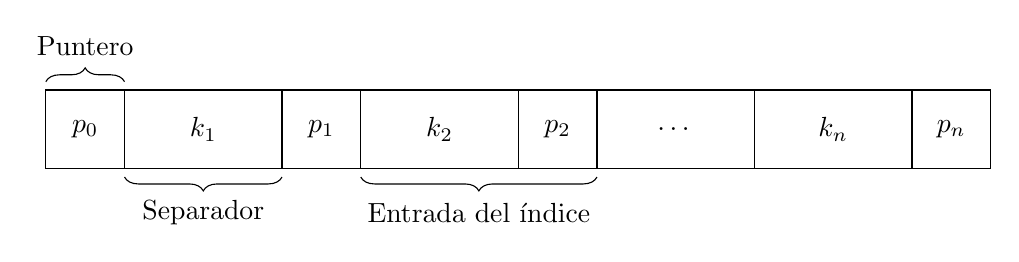
\begin{tikzpicture}
    \draw[draw=black] (0,0) rectangle (1,1) node[pos=.5] {$p_0$};
    \draw[draw=black] (1,0) rectangle (3,1) node[pos=.5] {$k_1$};
    \draw[draw=black] (3,0) rectangle (4,1) node[pos=.5] {$p_1$};
    \draw[draw=black] (4,0) rectangle (6,1) node[pos=.5] {$k_2$};
    \draw[draw=black] (6,0) rectangle (7,1) node[pos=.5] {$p_2$};
    \draw[draw=black] (7,0) rectangle (9,1) node[pos=.5] {\ldots};
    \draw[draw=black] (9,0) rectangle (11,1) node[pos=.5] {$k_n$};
    \draw[draw=black] (11,0) rectangle (12,1) node[pos=.5] {$p_n$};
    
    \draw [decorate,decoration={brace,amplitude=5pt,raise=4ex}] (0,.5) -- (1,.5) node[midway,yshift=3em]{Puntero};
    \draw [decorate,decoration={brace,amplitude=5pt,raise=4ex,mirror}] (1,.5) -- (3,.5) node[midway,yshift=-3em]{Separador};
    \draw [decorate,decoration={brace,amplitude=5pt,raise=4ex,mirror}] (4,.5) -- (7,.5) node[midway,yshift=-3em]{Entrada del índice};
  \end{tikzpicture}
  \caption{Ejemplo de página de un índice ISAM}
\end{figure}

Aquí siempre se tiene que cumplir que cuando un puntero $p_i$ apunta a un valor $k$.

\begin{figure}[h]
  \centering
  \begin{tikzpicture}
    \draw[draw=black] (0,0) rectangle (1,1) node[pos=.5] {$p_i$};
    \draw[draw=black] (-1,0) rectangle (0,1) node[pos=.5] {$k_i$};
    \draw[draw=black] (1,0) rectangle (2,1) node[pos=.5] {$k_{i+1}$};

    \draw[draw=black] (0,-1) rectangle (1,-2) node[pos=.5] {$k$};

    \draw[-Stealth] (.5,0) -- (.5,-1);
  \end{tikzpicture}
\end{figure}

se debe dar que $k_i \leq k \leq k_{i+1}$.

\subsubsection{Búsqueda en ISAM}
Hacer búsqueda en ISAM es muy similar a las búsquedas que se hacen en árboles.

\begin{algorithm}
  \caption{busquedaEnArbol($k$, $P$)}
  \KwIn{Una search key $k$ y una página $P$ del índice}
  \KwOut{Una página de datos que puede contener a $k$}
  \If{$P$ es una página de datos}{
    \Return $P$
  }
  $P = p_0 k_1 p_1 \ldots k_n p_n$\;
  \Switch{$k$}{
    \lCase{$k < k_1$}{\Return busquedaEnArbol($k$, $p_0$)}
    \lCase{$k_i \leq k < k_{i+1}$}{\Return busquedaEnArbol($k$, $p_i$)}
    \lCase{$k_n < k$}{\Return busquedaEnArbol($k$, $p_n$)}
  }
  
\end{algorithm}

\subsubsection{Range Queries en ISAM}
Para hacer una range query con valores entre \texttt{x} e \texttt{y}, considerando que tenemos el algoritmo escrito anteriormente
\begin{enumerate}
  \item Llamar $P = \texttt{busquedaEnArbol(x, root)}$.
  \item Realizar una busqueda binaria del mayor elemento $k^*$ en $P$ tal que $k^* \leq \texttt{x}$.
  \item Hacer scan desde $k^*$ sobre todos los valores menores o iguales a \texttt{y}
\end{enumerate}

\subsubsection{Inserción en ISAM}
Para insertar un valor $k$ en la página de índice $P$
\begin{enumerate}
  \item Llamar $P = \texttt{busquedaEnArbol($k$, root)}$.
  \item Si $P$ tiene espacio para $k$, insertar $k$ en $P$.
  \item Si $P$ no tiene espacio para $k$, insertar $k$ en una pagina de overflow.
\end{enumerate}

\subsubsection{Eliminación en ISAM}
Para eliminar un valor $k$
\begin{enumerate}
  \item Llamar $P = \texttt{busquedaEnArbol($k$, root)}$.
  \item Si $P$ contiene a $k$, eliminar $k$ en todas las páginas de overflow que contengan a $k$ (duplicados).
\end{enumerate}

\subsubsection{Costos de ISAM}
Considerando
\begin{itemize}
  \item $H$: Cantidad de niveles del arbol ISAM.
  \item $V$: Largo máximo de las cadenas de páginas de overflow.
\end{itemize}

Los costos para las operaciones vistas quedan en
\begin{itemize}
  \item Búsqueda: $\mathcal{O}(H + V)$
  \item Inserción: $\mathcal{O}(H + V)$
  \item Eliminación: $\mathcal{O}(H + V)$
\end{itemize}

\subsubsection{Pros y contras de ISAM}
\begin{itemize}
  \item \textbf{Pros}
  \begin{itemize}
    \item Rendimiento pobre si se realizan muchas modificaciones a los datos guardados.
    \item Deficiente si la cantidad de datos aumenta.
  \end{itemize}
  \item \textbf{Contras}
  \begin{itemize}
    \item Eficiente en búsqueda dentro de bases de datos con pocas modificaciones a sus datos.
    \item Sencillo de implementar.
    \item Útil para acceso concurrente.
  \end{itemize}
\end{itemize}


\subsection{B+-Trees}
Este es un tipo de índice muy similar a ISAM, pero a diferencia de este, B+-Trees no usa páginas de overflow y el árbol siempre está balanceado, logra mantener la eficiencia de la búsqueda ($\mathcal{O}(\#\text{tuplas})$) y usa procedimientos eficientes para insertar y eliminar elementos.

La forma que tienen los nodos es casi idéntica a ISAM
\begin{figure}[h]
  \centering
  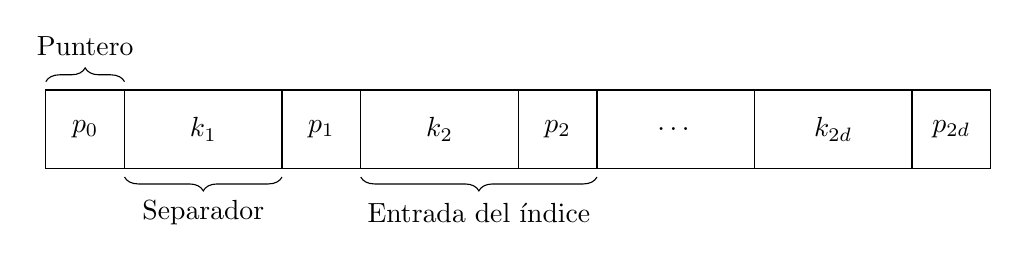
\begin{tikzpicture}
    \draw[draw=black] (0,0) rectangle (1,1) node[pos=.5] {$p_0$};
    \draw[draw=black] (1,0) rectangle (3,1) node[pos=.5] {$k_1$};
    \draw[draw=black] (3,0) rectangle (4,1) node[pos=.5] {$p_1$};
    \draw[draw=black] (4,0) rectangle (6,1) node[pos=.5] {$k_2$};
    \draw[draw=black] (6,0) rectangle (7,1) node[pos=.5] {$p_2$};
    \draw[draw=black] (7,0) rectangle (9,1) node[pos=.5] {\ldots};
    \draw[draw=black] (9,0) rectangle (11,1) node[pos=.5] {$k_{2d}$};
    \draw[draw=black] (11,0) rectangle (12,1) node[pos=.5] {$p_{2d}$};
    
    \draw [decorate,decoration={brace,amplitude=5pt,raise=4ex}] (0,.5) -- (1,.5) node[midway,yshift=3em]{Puntero};
    \draw [decorate,decoration={brace,amplitude=5pt,raise=4ex,mirror}] (1,.5) -- (3,.5) node[midway,yshift=-3em]{Separador};
    \draw [decorate,decoration={brace,amplitude=5pt,raise=4ex,mirror}] (4,.5) -- (7,.5) node[midway,yshift=-3em]{Entrada del índice};
  \end{tikzpicture}
\end{figure}

La diferencia es que la cantidad máxima de llaves y punteros ($n$) está definida por el orden del árbol ($d$) B+-Tree
\begin{align*}
  d &\leq n \leq 2d\\
  1 &\leq n \leq 2d \quad \text{para root}
\end{align*}

Este orden $d$ es siempre el orden del tamaño de una página.
\[ d \approx \frac{B}{2} \]

Para buscar en un B+-Tree, el algoritmo de búsqueda es exactamente el mismo que en ISAM.

\subsubsection{Range Queries en B+-Trees}
Para hacer una range query entre \texttt{x} e \texttt{y}, considerando que tenemos \texttt{busquedaEnArbol($k$, $P$)}.
\begin{enumerate}
  \item Llamar $P = \texttt{busquedaEnArbol(x, root)}$.
  \item Realizar una busqueda binaria del mayor elemento $k^*$ en $P$ tal que $k^* \leq \texttt{x}$.
  \item Hacer scan desde $k^*$ sobre todos los valores menores o iguales a \texttt{y}
\end{enumerate}

\makeobservationbox{Supuesto}{Se asume que todos los data keys son diferentes (sin duplicados)}

\subsubsection{Inserción en B+-Trees}
Para insertar un valor $k$
\begin{enumerate}
  \item Llamar $P = \texttt{busquedaEnArbol($k$, root)}$.
  \item Si el espacio libre de $P$ es menor o igual a $2d$, insertar $k$ en $P$.
  \item Si no es así, se debe insertar $k$ en $P$, y luego hacer split de $[P + k]$, donde $[P + k] = k_1^* k_2^* \ldots k_{2d}^* k_{2d+1}^*$ (es una página de datos).
\end{enumerate}

Para hacer split de una página de datos $[P + k]$ de tamaño $2d + 1$
\begin{enumerate}
  \item Asuma $[P + k] = k_1^* k_2^* \ldots k_{2d}^* k_{2d+1}^*$ con $k_i < k_{i+1}$.
  \item Divida $[P + k]$ en dos páginas
  \[ P_1 = k_1^* \ldots k_d^* \quad P_2 = k_{d+1}^* \ldots k_{2d+1}^* \]
  y reemplace $P$ por $P_1, P_2$ en la lista doble-ligada de datos.
  \item Seleccione el valor $k_{d+1}$ como divisor de $P_1$ y $P_2$.
  \item Reemplace el puntero $p$ en la página $P'$ que apuntaba a la página $P$ por $p_1 k_{d+1} p_2$ donde $p_1$ apunta a $P_1$ y $p_2$ apunta a $P_2$.
  \item Itere sobre la página de directorio $P'$ que apuntaba a $P$ (split de $P'$).
\end{enumerate}

Para hacer split de una página de directorio $P$ de tamaño $2d + 1$
\begin{enumerate}
  \item Asuma $P = k_1 k_2 \ldots k_{2d} k_{2d+1}$ con $k_i < k_{i+1}$.
  \item Divida $P$ en dos páginas
  \[ P_1 = k_1 \ldots k_d \quad P_2 = k_{d+1} \ldots k_{2d+1} \]
  y reemplace $P$ por $P_1, P_2$ en el directorio.
  \item Seleccione el valor $k_{d+1}$ como divisor de $P_1$ y $P_2$.
  \item Reemplace el puntero $p$ en la página $P'$ que apuntaba a la página $P$ por $p_1 k_{d+1} p_2$ donde $p_1$ apunta a $P_1$ y $p_2$ apunta a $P_2$.
  \item Itere sobre la página de directorio $P'$ que apuntaba a $P$ (split de $P'$).
\end{enumerate}

Para hacer split del nodo raíz de un B+-Tree, se comienza haciendo split en las hojas y continúa hasta llegar a la raíz. Si es necesario hacer split de todos los nodos y el nodo raíz está lleno, entonces será necesario crear un nuevo nodo raíz. Una consecuencia de esto, es que la profundidad del árbol aumentará.

\subsubsection{Eliminación en B+-Trees}
Para eliminar un valor $k$
\begin{enumerate}
  \item Llamar $P = \texttt{busquedaEnArbol($k$, root)}$.
  \item Si el espacio usado en $P$ es mayor o igual a $d+1$, eliminar $k$ en $P$.
  \item Si no, se debe eliminar $k$ en $P$ y rebalancear $[P + k]$
\end{enumerate}

\subsubsection{Costos de B+-Trees}
Considerando
\begin{itemize}
  \item $T$: Número de túplas.
  \item $B$: Tamaño de una página.
\end{itemize}

Los costos para las operaciones vistas quedan en
\begin{itemize}
  \item Búsqueda: $\mathcal{O}(\log_{\frac{B}{2}}(\frac{2 \cdot T}{B}))$
  \item Inserción: $\mathcal{O}(\log_{\frac{B}{2}}(\frac{2 \cdot T}{B}))$
  \item Eliminación: $\mathcal{O}(\log_{\frac{B}{2}}(\frac{2 \cdot T}{B}))$
\end{itemize}

\subsubsection{Lidiando con elementos duplicados en B+-Trees}
Antes se habia hecho la suposición de que no estabamos trabajando con elementos duplicados jamás. Sin embargo, esto es algo que claramente puede ocurrir. Si consideramos elementos duplicados, se tienen varias opciones.
\begin{itemize}
  \item Usar páginas de overflow.
  \item Entradas con llaves compuestas.
  \item Permitir duplicados y flexibilizar los intervalos del directorio.
  \[ k_i \leq k < k_{i+1} \Rightarrow k_i \leq k \leq k_{i+1} \]
\end{itemize}

\section{Índices basados en Hashing}
Los índices basados en hashing almacenan la información del índice por medio de una tabla de hash y una función de hashing. Estos índices son muy eficientes para hacer consultas de valores, aunque no son tan eficientes para range queries como lo es B+-Trees. A día de hoy, la mayoría de motores de bases de datos incluyen soporte para hash indexes.

\subsection{Static Hashing}
En Static Hashing, el índice es almacenado usando una tabla de hash, en donde se tienen $N$ buckets (páginas en disco). Cada bucket tiene una lista ligada de overflow pages. Para relacionar las entradas del índice con su valor correspondiente, se usa una función de hash $h: \texttt{datatype}(X) \rightarrow [0, \ldots, N-1]$.

\begin{figure}[h]
  \centering
  \begin{tikzpicture}
    \draw[draw=black] node (k) (0,0) {$k$};
    \draw[draw=black] (3,0) circle (10pt) node[] (h) {$h$};
    \draw[draw=black] (5,2) rectangle (7,-2);
    \draw[draw=black] (5.5,1.75) rectangle (6.5,1.25) node[pos=.5] (zero) {$0$};
    \draw[draw=black] (5.5,.75) rectangle (6.5,.25) node[pos=.5] (one) {$1$};
    \draw[draw=black] (5.5,-.25) rectangle (6.5,-.75) node[pos=.5] (dots) {$\ldots$};
    \draw[draw=black] (5.5,-1.25) rectangle (6.5,-1.75) node[pos=.5] (last) {$N-1$};
    \draw[draw=black] (7.5,-1.25) rectangle (9,-1.75) node[pos=.5] (over) {Overflow};

    \draw [-Stealth] (.25,0) -- (2.6,0);
    \draw [-Stealth] (3.4,0) -- (5.5,1.5);
    \draw [-Stealth] (3.4,0) -- (5.5,.5);
    \draw [-Stealth] (3.4,0) -- (5.5,-.5);
    \draw [-Stealth] (3.4,0) -- (5.5,-1.5);
    \draw [-Stealth] (6.5,-1.5) -- (7.5,-1.5);
  \end{tikzpicture}
  \caption{Funcionamiento de la función de hashing}
\end{figure}

\subsubsection{Operaciones en static hashing}
Para buscar, insertar y eliminar una llave $k$
\begin{enumerate}
  \item Computar el valor $h(k)$.
  \item Acceder al bucker en la posición $h(k)$.
  \item Buscar / Insertar / Eliminar la tupla en la página $h(k)$ o sus overflow pages.
\end{enumerate}

\subsubsection{Colisiones}
Puede llegar a pasar que para la función de hashing $h(k)$, existan dos valores $k_1 \not= k_2$, pero que $h(k_1) = h(k_2)$. Idealmente se debe encontrar una función de hashing en donde las colisiones sean disminuidas al mínimo. Idealmente, la función de hash se debería comportar de forma aleatoria para $k_1, \ldots, k_n$.

\subsubsection{Costo de operaciones}
Dada
\begin{itemize}
  \item Una buena selección de la función de hash $h$
  \item $\texttt{\#(data-entries)} \propto B \cdot N$, con $B$ tamaño de página y $N$ buckets.
\end{itemize}
se tiene que el costo de todas las operaciones es constante.
\[ \approx \frac{\texttt{\#(data-entries)}}{B \cdot N} \]

\subsection{Extendable Hashing}
La idea es usar un directorio de buckets principales, y luego duplicar el tamaño del directorio cuando haya un overflow de un bucket.

\begin{figure}[h]
  \centering
  \begin{tikzpicture}
    \draw[draw=black] node (0,0) (k) {$k$};
    \draw[draw=black] (3,0) circle (10pt) node[] (h) {$h$};
    \draw[draw=black] (5,2) rectangle (7,-2);
    \draw[draw=black] (5.75,2.5) rectangle (6.25,2) node[midway, midway] {2};
    \draw[draw=black] (5.5,1.75) rectangle (6.5,1.25) node[pos=.5] (00) {$00$};
    \draw[draw=black] (5.5,.75) rectangle (6.5,.25) node[pos=.5] (01) {$01$};
    \draw[draw=black] (5.5,-.25) rectangle (6.5,-.75) node[pos=.5] (10) {$10$};
    \draw[draw=black] (5.5,-1.25) rectangle (6.5,-1.75) node[pos=.5] (11) {$11$};
    
    \draw[draw=black] (7.5,1.75) rectangle (10,1.25) node[pos=.5] (bucket1) {$4^*, 10^*, 12^*, 38^*$};
    \draw[draw=black] (7.5,0.25) rectangle (10,-0.25) node[pos=.5] (bucket2) {$1^*, 5^*, 21^*$};
    \draw[draw=black] (7.5,-1.25) rectangle (10,-1.75) node[pos=.5] (bucket3) {$15^*, 7^*, 19^*$};

    \draw[draw=black] (10,1.75) rectangle (10.5,1.25) node[pos=.5] {1};
    \draw[draw=black] (10,0.25) rectangle (10.5,-0.25) node[pos=.5] {2};
    \draw[draw=black] (10,-1.25) rectangle (10.5,-1.75) node[pos=.5] {2};

    \draw [-Stealth] (k.east) -- ([xshift=-5pt]h.west);
    \draw [-Stealth] (h)+(10pt,0) -- ([xshift=-5]00.west);
    \draw [-Stealth] (h)+(10pt,0) -- ([xshift=-5]01.west);
    \draw [-Stealth] (h)+(10pt,0) -- ([xshift=-5]10.west);
    \draw [-Stealth] (h)+(10pt,0) -- ([xshift=-5]11.west);
    % \draw [-Stealth] (3.4,0) -- (5.5,.5);
    % \draw [-Stealth] (3.4,0) -- (5.5,-.5);
    % \draw [-Stealth] (3.4,0) -- (5.5,-1.5);
    \draw [-Stealth] ([xshift=5]00.east) -- (bucket1.west);
    \draw [-Stealth] ([xshift=5]01.east) -- (bucket1.west);
    \draw [-Stealth] ([xshift=5]10.east) -- ([xshift=-10]bucket2.west);
    \draw [-Stealth] ([xshift=5]11.east) -- ([xshift=-10]bucket3.west);
  \end{tikzpicture}
  \caption{Extendable hashing}
\end{figure}

\subsubsection{Inserción en Extendable Hashing}
\begin{enumerate}
  \item Computamos $h_n(k)$.
  \item Buscamos en el directorio el puntero $p$ para la entrada $h_n(k)$.
  \item Seguimos el puntero $p$ al buscket $B$ correspondiente.
  \item Si hay espacio en $B$, insertamos $k$ en $B$.
  \item Si no hay espacio en $B$ con profundidad local $d$, se debe realizar un bucket split de $B$. Así, se aumenta la profundidad local de $B_0$ y $B_1$ a $d+1$.
  \begin{itemize}
    \item Si $n>d$, insertamos $B_0$ y $B_1$ en el directorio.
    \item Si $n=d$, hacemos un doblamiento del directorio.
  \end{itemize}
\end{enumerate}

\subsubsection{Bucket Split}
Dado un bucket $B$ con profundidad local $d$, se dividen sus elementos en dos buckets según el bit $d+1$.

\subsubsection{Doblamiento del Directorio}
Dado un bucket $B$ con profundidad local $d=n$, hacemos un bucket split de $B$ y duplicamos el tamaño del directorio a $2^{n+1}$.

\subsubsection{Eliminación en Extendable Hashing}
Para eliminar un elemento $k*$, este se debe buscar y eliminar del bucket al que pertenezca. Si el bucket queda vacío, extendable hashing hace merge de buckets, aunque esto es poco usado.

\subsubsection{Costo de Extendable Hashing}
Considerando $D$ el tamaño del directorio en páginas, el costo de cada operación es
\begin{itemize}
  \item Búsqueda: $\mathcal{O}(1)$
  \item Inserción: $\mathcal{O}(D)$
\end{itemize}

\section{Índices Multidimensionales - Bitmap Index}
En los índices multidimensionales, existe más de una search key en una misma tupla, con todas esas search key con el mismo grado de importancia.

Bitmap index es un índice multidimensional bastante diferente al resto de propuestas que existen. Permite realizar consultas multidimensionales y está basado en una codificación alternativa de las tuplas de una relación.

Para una relación $R$
\begin{enumerate}
  \item Enumeramos sus tuplas del 1 a $|R|$ de forma permanente, donde $R = \{ t_1, t_2, \ldots, t_{|R|} \}$.
  \item Para un atributo $c$ de $R$ y un valor $v \in \pi_c(R)$ definimos un string binario $b_v^c$ de largo $|R|$ tal que
  \[ 
    b_v^c[i] = 
    \begin{cases} 
      1 & \text{si } t_i(c) = v\\
      0 & \text{en otro caso.}
    \end{cases}
  \]
  \item Un bitmap index sobre un atributo $c$ se define como el conjunto $B^c = \{ b_v^c | v \in \pi_c(R) \}$
\end{enumerate}

Bitmap index es muy útil para consultas con filtros complejos, columnas de baja cardinalidad y datos que sufren pocas modificaciones. Por otro lado, es bastante deficiente cuando los datos requieren ser actualizados frecuentemente.

